
%%%%%%%%%%%%%%%%%%%%%%% file typeinst.tex %%%%%%%%%%%%%%%%%%%%%%%%%
%
% This is the LaTeX source for the instructions to authors using
% the LaTeX document class 'llncs.cls' for contributions to
% the Lecture Notes in Computer Sciences series.
% http://www.springer.com/lncs       Springer Heidelberg 2006/05/04
%
% It may be used as a template for your own input - copy it
% to a new file with a new name and use it as the basis
% for your article.
%
% NB: the document class 'llncs' has its own and detailed documentation, see
% ftp://ftp.springer.de/data/pubftp/pub/tex/latex/llncs/latex2e/llncsdoc.pdf
%
%%%%%%%%%%%%%%%%%%%%%%%%%%%%%%%%%%%%%%%%%%%%%%%%%%%%%%%%%%%%%%%%%%%


\documentclass[runningheads]{llncs}
\usepackage{amsmath}
\usepackage{mathtools}
\usepackage{amssymb}
\usepackage{float}
\usepackage{multicol}

\setcounter{tocdepth}{3}
\usepackage{graphicx}
\usepackage[sorting=none]{biblatex}
\addbibresource{references.bib}



\usepackage{url}
\urldef{\mailsc}\path||
\newcommand{\keywords}[1]{\par\addvspace\baselineskip
\noindent\keywordname\enspace\ignorespaces#1}

\begin{document}

\mainmatter  % start of an individual contribution

% first the title is needed
\title{Application of a chain-like and a hypercube communication topologies 
in a multi-swarm PSO algorithm applied to continuous optimization problems}
% Los titulos no llevan punto al final - M
% Maybe this is a bit too long? Also, it would be best to say *why*
% you did this, instead of what you did - JJ

% a short form should be given in case it is too long for the running head
\titlerunning{Appli. of comm. topologies in multi-swarm PSO}

% the name(s) of the author(s) follow(s) next
%
% NB: Chinese authors should write their first names(s) in front of
% their surnames. This ensures that the names appear correctly in
% the running heads and the author index.
%
\author{José Guzmán \and Mario García-Valdez \and Juan J. Merelo-Guervós}

\authorrunning{Guzmán et al.}
% (feature abused for this document to repeat the title also on left hand pages)

% the affiliations are given next; don't give your e-mail address
% unless you accept that it will be published
\institute{Tijuana Institute of Technology, Tijuana, Mexico
  \email{jose.guzmanc19@tectijuana.edu.mx, mario@tectijuana.edu.mx} \and
University of Granada, Spain, \email{jmerelo@ugr.es}}



%
% NB: a more complex sample for affiliations and the mapping to the
% corresponding authors can be found in the file "llncs.dem"
% (search for the string "\mainmatter" where a contribution starts).
% "llncs.dem" accompanies the document class "llncs.cls".
%

\toctitle{}
\tocauthor{José Guzmán, Mario García-Valdez}

\maketitle


\begin{abstract}

  Using multiple-swarm PSO is a technique used in recent years to help improve
  the performance of nature-inspired optimization algorithms. A distributed PSO
  algorithm can work in each swarm in parallel and also communicate particles
  between them asynchronously. However, the design of these systems is not a
  trivial task because many architectural options affect the exploration and
  exploitation of the search space. In this paper, we focus on proposing and
  comparing two communication policies regarding which swarms can communicate
  with each other. These policies intend to limit the communication between
  populations to increase exploration and avoid premature convergence. The
  proposed policies are chain and hypercubic topologies. We implemented them
  following an event-based cloud-native design. We compared the three options
  using several continuous optimization benchmark functions to assess the
  benefits of changing a communication topology. After the experiments, the
  chain topology had a better performance using MSE as a metric.
  % Probably rewrite it. Why did you do it? Why did
                  % you think it would work? - JJ
 % Done - Mario 
 % Edit at will - Mario


\keywords{PSO, EvoSwarm, multi-swarm intelligence, communication topologies,
 chain algorithm, hypercube, multi-swarm PSO.}
\end{abstract}


\section{Introduction}

% 1. State the context
% 2. State the problem
% 3. Say the hypothesis you want to prove in the paper, its objective.
% 4. Say how you want to prove that hypothesis.

Among the various strategies that have emerged in recent times for bio-inspired
optimization algorithms, the creation of multiple populations working
in parallel and (possibly) asynchronously has proven to be valuable in 
solving complex optimization problems \cite{a1}.
Researchers often divide the original population into small sub-populations in order to 
achieve a certain outcome, for instance, solving large-scale optimization problems and dynamic
optimization problems. There are some studies on multi-population optimization that show
that it is possible integrate this aproach easily into various nature-inspired optimization algorithms,
and often outperforms the ones using single-population optimization algorithms \cite{b11} \cite{b12}.
Other investigations, reviews, and surveys on multi-population approaches have also
been published in recent years, in which multi-population concepts are described
using other terms like 'parallel,' 'Cooperative,' 'co-evolution,' and 'islands.'
Its multi-threaded and parallel processing features that significantly speed up
deployment time \cite{b13} \cite{b14}.

One of the critical points in this technique is communication between
populations, since it has been observed in various studies that the
exchange of possible solutions helps optimizations algorithms to gain performance \cite{a2}. The following four parameters
control communication between sub-populations:

\begin{itemize}
    \item A communication speed that defines how many solutions are able to be exchanged between sub-populations.
    \item A communication policy encharge of selecting which solutions should be replaced by those of coming from another sub-populations.
    \item A communication interval that establishes the frequency to execute the communication.
    \item A connection topology that specifies the exact way subpopulations communicate.
\end{itemize}

Several distributed architectures have been proposed to manage the communication
and parallel execution of these kind of algorithms, for example there is a
similar approach by Scott Haberson et al. using a multi-population parallel
genetic algorithm for independent evolution \cite{da1}. 

In this paper, we propose the two communication topologies to be implemented in a 
even-based distributed multi-swarm Particle Swarm Optimization (PSO) algorithm.
These comminication topologies follow a chain and a hypercube structure on a milti-swarm. We chose
these topologies for their ability to be adapted to the architecture
mentioned above. They can work without altering the optimization
algorithm allowing a fair comparison with other communication
methods. 

This paper contains the following sections: We present state-of-the-art on
multi-swarm optimization in Section 2. In Section 3, we present two variants of communication topologies,
to be used in an event-based architecture we also present in the section. In Section 4, 
we describe the experimental setup and results, Furthermore,
Section 5 presents the conclusions for this work.

\section{State of the Art}

Particle Swarm Optimization (PSO) is an optimization algorithm
inspired by the collective behavior of some flocks of birds or schools of fish. It was introduced in 1995 by  J. Kennedy and
R. Eberhar, it has undergone several improvements \cite{b1}. % pon el nombre del autor - M -j
Since then, researchers have created different versions, which aimed at different
purposes, developed new applications in various areas, published many studies on the effects of various parameters, and proposed great variety algorithm variants \cite{b2}. A basic version of the PSO algorithm
works with a population , called a swarm, of possible solutions
known as particles. These ones move in the search space according to
some simple rules derived from formulas. The movements in the particles' search space are
determined by their best known locations and by the best known location
of the entire swarm. These locations are suppossed to get better and they will
guide the swarm's movements. The process is repeated many times, so it
is expected that solution that meets the requirements will eventually be
discovered, although this may not happen\cite{b3}.



Multi-swarm optimization is one of the most known variants of Particle Swarm Optimization
(PSO) based the creation of multiple swarms (or sub-swarm) instead of just one. The basic flow in
a multi-swarm optimization is that each sub-swarm has it's own specific region to concentrate. A specific diversification method decides where and
when to locate and execute this sub-swarms.

For example, Wave of Swarm of Particles \cite{b6} uses a technique on the "collision" of particles. When the
particles are close to each other, they are sent into new sub-swarms,
preventing full convengece between the sub-swarms. Another examples is the Dynamic Multi-Swarm-Particle
Swarm Optimizer\cite{b7} that rearranges the particles from the sub-swarms
(when converged) into new ones periodically, so the new
iteration of sub-swarms have the advantage of starting with particles from the previous
one. Locust swarms \cite{b8} are founded on a "devour and go" strategy
after a sub-swarm consumes or "devours" a small fraction of the search space an explorer is deployed to search for
new regions making the sub-swarm move to the new promised location ("keep going").

In contrast to typical PSO swarms, sub-swarms are fed with information about
previous swarms. These could be the positions and velocities instead of having
their initial parameters to be randomly selected. Generaly speaking, the development of
multi-swarm systems creates a new path of design options that who were not present at the time the original PSO emerged. 
These design decisions now have guidelines thanks to the numerous studies on the topic, for
example, tow common opotions are the use of non-random initial positions and initial velocities for the particles in the subs-warms helping to
better results, which is not the case for individual swarms \cite{b9}.

A few number of this options can be reached by relatively independent
subcomponents that allow different aproaches to this matter to be
tested. For example, the multi-swarm system UMDA-PSO \cite{b10} 
applies a multi-swarm hybrid aproach using a diverse combination of 
elements from particle swarm optimization, distribution estimation 
algorithm, and differential evolution.

% Rewrite this too -- JJ
There have been some papers focused in optimizing the communication
between swarms, for example the survey in reference \cite{b15} has a
collection of different investigations around this subject. For
example El-Abd and Kamel talked over the multiple factors that can
change the overall behavior of multiple joined swarms, some of this factors
were the strategy and path of comunications between swarms and the number sub-swarms. 
Then an experiment was made applying a circular topology of comunications, 
the results demonstrated that this aproach has an overall superior performance 
than using a simpler techniche of sharing the global best of all the swarms\cite{b16}. 

Another example and the source of inspiration for this paper, is one
of Li and Zeng, who presented a multi-population algorithm with a chain-like structure for parallel global
numerical optimization. In this aproximation a few changes where applied, like a dynamic neighborhood,
in order to improve the parallel optimization\cite{b17}. 

In the next section, we present two variants of communication topologies,
to be used in an event-based architecture for the implementation of 
distributed population-based optimization algorithms.


\section{Proposed method}

Recently, there is an interest in cloud-native, event-based architectures
suitable to run locally on a personal computer or in a cloud platform service.
An event-based architecture uses events to trigger and communicate between
services and processes. Using an event-based architecture, we intend to carry
out a series of experiments to analyze the effect of changing the communication
topology in a multi-population optimization algorithm's performance. Using this
type of architecture with a multi-swarm optimization algorithm is a new
approach. Therefore, there is an opportunity to find a substantial variation in
the performance of such an optimization algorithm by changing the way the
various swarms communicate to exchange information.

\subsection{EvoSwarm} 
First, we briefly present the overall architecture of EvoSwarm, the 
platform in which we implemented the distributed algorithm. 

EvoSwarm follows an event-based architecture, using message queues for
interprocess communication. Messages consist of small populations or swarms that
are consumed by worker processes that run a local PSO for a small number of
iterations. After this, the resulting swarm is pushed to another message queue
to be consumed by a migration process responsible for the communication
(migration) between swarm messages kept in a buffer \cite{b18}.
% Better a higher-level description, describing what's in
            % the queues. Also, message queues. - JJ

            % (See Figure \ref{fig:example}).

% \begin{figure}[h]
% \centering
% \DeclareGraphicsExtensions{.jpg}
% 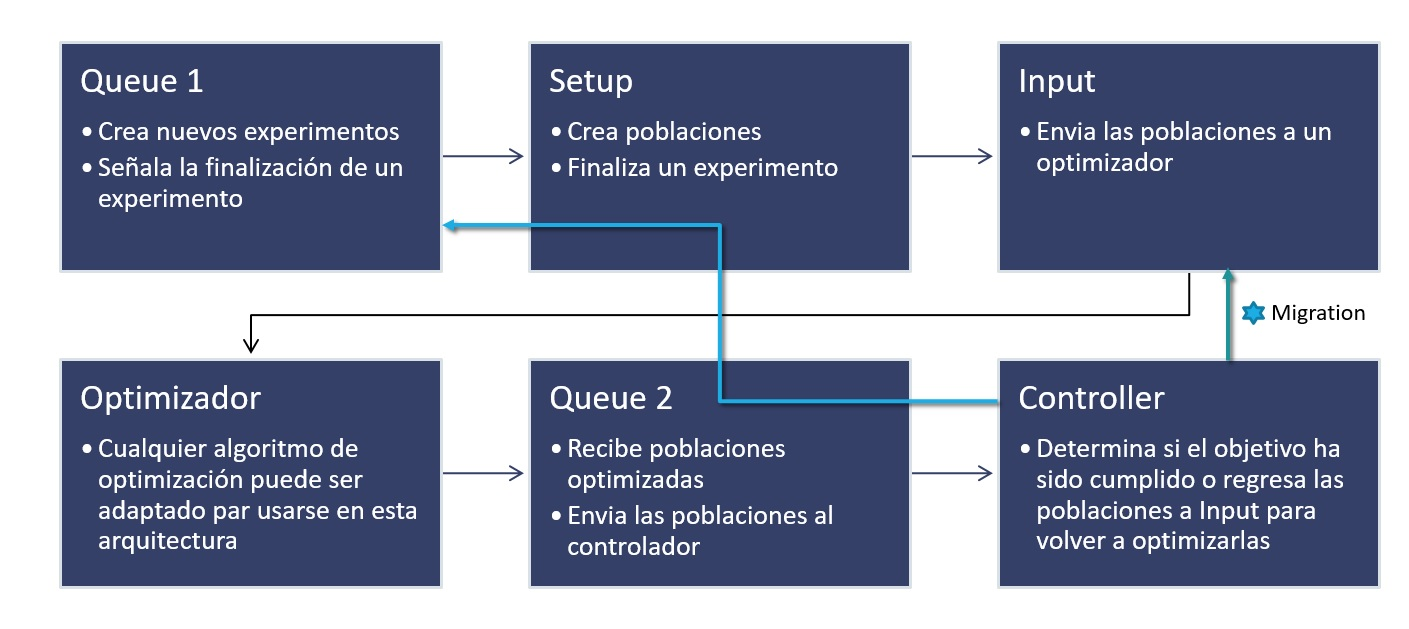
\includegraphics[scale=.40]{Resources/F1-1.jpg}
% \caption{The EvoSwarm flow.}
% \label{fig:example}
% \end{figure}
% Eliminated. It's in Spanish...

It is worth mentioning that this architecture can be implemented using various
computers in a network or using virtualization, in work we used Docker containers. 
Here are some of the most important features that
EvoSwarm brings to the user:

\begin{itemize} 
  
  \item Fully capable of scalability, since more computers can be added to the
  network in order to manage a more significant workload.
    
    \item Independence between processes, which means that any process in the
    structure is completely separated from the other ones allowing more work to
    be done at the same time.
    
    \item It is adaptable to any population-based optimizing algorithm.
\end{itemize}

The only change made to the original version of EvoSwarm \cite{b18} was the
communication policy between the populations of the multi-swarm PSO.

\subsection{Proposed communication topologies for EvoSwarm} 

In the original communication policy, the architecture waited until a minimum of
three populations reached the migration component. These populations are sent to
a process that combines the best half of each one with the others. For example,
let us name the three populations A, B, and C, then a sort method is applied to
each one (based on the quality of the solution). The sorted populations are now
divided into halves in preparation for the merging process, now, with three new
populations, the first one has the best half of A and B, the second has the best
of B and C, and the third has the best of A and C. The last step is reinserting
these new populations into a queue from which the PSO processes will retake
them.

The first modification, in this case, is only on the merging process. To create
a chained algorithm that affects every three arriving populations, we sort the
three populations. The modification consists in that the populations are only
allowed to share a few members of the elite. In this case, 10. Individuals are
carried into a chain structure in which a population can receive only one way of
the structure and shares in another.

The 2nd variation for the EvoSwarm structure is a hypercube; we based this one
on a paper in which this topology was applied to solve a multi-reservoir of
water using a multi-population algorithm \cite{b20}. The name indicates this
method has a cubic structure and can only function with eight populations or
more. For this paper, we only need eight populations. Once the algorithm gets
filled with eight populations, the migrations algorithm needs to assign each one
a place in the hypercube structure. Figure 3 it has shown the layout of the
structure.

The structure resembles a cube, and in every one of its vertices is one
population. One thing that stands immediately is the capital P because only four
populations have it. In this algorithm, we divided the hypercube into two
dimensions. Moreover, depending on the iteration of the experiment, the exchange
of solutions is restricted.

Every iteration of an experiment changes the mode in which the populations
communicate with each other. For example, in the first iteration, the eight
populations can only communicate with the others in the same dimension. In the
second iteration, the opposite happens, allowing them to exchange information
with a population outside that dimension. With eight vertices, only two
exchanges are allowed, and for the experiments on this paper, only the best 10\%
of solutions migrate to another swarm.


\section{Experimental Setup and Results}

We implemented the migration policies in Python; for the PSO algorithm, we use
the Evolopy library \cite{b19}, as mentioned earlier in this paper, we use the
same parameters for the PSO algorithm as the EvoSwarm paper (see Table 1).



\begin{table}[h!]
\centering
\caption{Parameters PSO of Evolopy libray}
\begin{tabular}{|c c|} 
 \hline
 Parameters & Values  \\ [0.5ex] 
 \hline\hline
 Vmax & 6 \\ 
 Wmax & 0.9 \\
 Wmin & 0.2 \\
C1 & 2 \\
C2 & 2 \\[0.5ex]
 \hline
\end{tabular}
\label{table:1}
\end{table}

Continuing with the configuration of the experiments, Table 2 presents the
parameters used in EvoSwarm; these are for the 3 cases presented in this paper.

\begin{table}[h]
\centering
\caption{Parameters for EvoSwarm}
\scalebox{0.90}{
\begin{tabular}{|c c c c c|} 
 \hline
 Dimensions & Generations  & Population size & Num. Experiments & Num. Population created\\ [0.2ex] 
 \hline\hline
 10 & 50 & 70 & 30 & 10 \\ 
 20 & 66 & 100 & 30 & 10 \\[0.2ex]
 \hline
\end{tabular}}
\label{table:1}
\end{table}

\subsection{Benchmark Functions}
%Aqui poner ref del pdf de coco

In order to run the optimization experiments, we selected ten functions from the
COCO benchmark. We selected these functions because in our preliminary
experiments, they showed performance variations as we changed the communication
topology. Here are the ten functions:

\begin{multicols}{2}
\begin{itemize}

    \item Function 1: Sphere.
    \item Function 2: Elipsoid separable.
    \item Function 3: Rastrigin separable.
    \item Function 9: Rosenbrock rota-ted.
    \item Functions 10: Elipsoid.
    \item Function 15: Rastrigin.
    \item Function 17: Schaffer F7, condition 10.
    \item Function 18: Schaffer F7, condition 1000.
    \item Function 21: Gallagher 101 peaks.
    \item Function 22: Gallagher 21 peaks

\end{itemize}
\end{multicols}

The number given to each function comes from COCO. This means that any method
using the benchmark can be compared against a great variety of optimization
methods. The complete collection of functions, graphics, and equations can be
reviewed in reference \cite{bbob}.

% Add some information about how the experiments were performed, type
% of machine, how much time they took ... -JJ

\subsection{Experimental Results}

We run the experiments in a single computer using a Ryzen 5 2600x CPU and 24 GB
of ram in Windows 10 Professional 64 bits, using Docker Desktop version 2.5,
running ten containers. We used Python version 3.5.7. We conducted each
experiment separately 30 times. The time required for each run took about 7
hours. In these experiments, we are not interested in the total time required to
find a solution as the changes in the algorithm did not affect the running time.
In this case, we are focused on the MSE of the best solution found with the same
number of function evaluations.

In ten dimensions, there are three functions in which the original topology
gives better results than the topologies we propose (shown in boldface).
However, once we reach twenty dimensions, the original topology obtains the
worst results. Overall the chain topology gives a better MSE in 20 dimensions,
only having two cases with a lower MSE than the hypercube configuration. We can
see that the standard deviation of the MSE obtained by the three options only
varies in few cases.In particular, the function $f_{10}$ was difficult for this
algorithm and could not find a target in any run.  

In the same table, we present the results of the statistical tests of comparing
both topologies against the original migration. In this case, we use a \(Z\)
statistical test with an $\alpha$ of 0.5, giving a critical value of 1.64.
Underline results have sufficient statistical evidence to have less MSE; this
means that changing the communication topology can improve, in some cases, the
performance of a multi-population optimization algorithm.


% Also, % you need to comment these results JJ % Also,
% you need to comment these results JJ
% ok - M 

\begin{table}[h!tb]
    \centering
    \caption{Comparison between the MSE obtained from 30 runs. We show the best results in boldface. Also, we
     present the statistical comparison against the EvoSwarm method, with significant results underlined. }
    \scalebox{0.72}{
    \begin{tabular}{|c|c||c|c|c||c|c|c|}
    \hline
     Dimensions & Function & EvoSwarm MSE & Chain MSE & Hypercube MSE & EvoSwarm Stdev & Chain Stdev & Hypercube Stdev \\ [0.5ex] 
    \hline\hline
10	&	1	  &	4.78611E-09	          &	\textbf{4.45791E-09}	&	4.52861E-09	&	3.3503E-09	&	3.27217E-09	&	3.25265E-09	\\
10	&	2	  &	\textbf{3.83054E-09}	&	4.1792E-09	&	4.65155E-09	&	2.35352E-09	&	2.86765E-09	&	2.9481E-09	\\
10	&	3	  &	2.352927573	          &	 \underline{\textbf{0.537649443}}	&	\underline{0.805637277}	&	2.881847604	&	1.543574882	&	1.663900202	\\
10	&	9	  &	0.49249742	          &	0.2527938	&	\textbf{0.229809004}	&	0.983944824	&	0.152990827	&	0.109927138	\\
10	&	10	&	\underline{\textbf{250.1738327}}	&	430.5420728	&	374.4359744	&	228.3598149	&	527.2651437	&	323.3050765	\\
10	&	15	&	14.66500256	          &	\underline{\textbf{12.05469416}}	&	13.33777036	&	6.840266769	&	5.391630829	&	5.860112176	\\
10	&	17	&	0.0923583	&	\textbf{0.075762972}	&	0.087059177	&	0.16646265	&	0.155990531	&	0.17433065	\\
10	&	18	&	0.524852914	&	0.506412719	&	\textbf{0.413659866}	&	0.633592264	&	0.467805944	&	0.382221237	\\
10	&	21	&	0.329852279	&	0.237422927	&	\textbf{0.20667313}	&	0.621910649	&	0.481633605	&	0.390914491	\\
10	&	22	&	0.692064149	&	\textbf{0.514782111}	&	0.57179096	&	0.577929599	&	0.719118705	&	0.650216016	\\
20	&	1	&	0.03594249	&	5.55231E-09	&	\textbf{5.54663E-09}	&	0.196865099	&	2.9048E-09	&	2.52356E-09	\\
20	&	2	&	5.64673E-09	&	5.49755E-09	&	\textbf{5.36566E-09}	&	2.31813E-09	&	2.54807E-09	&	2.98753E-09	\\
20	&	3	&	12.082746	&	8.746638682	&	\underline{\textbf{7.874205319}}	&	8.54691241	&	7.803681637	&	7.808562704	\\
20	&	9	&	\textbf{11.10349719}	&	11.37025195	&	11.49485451	&	1.483577297	&	2.321860001	&	1.0945346	\\
20	&	10	&	4994.888993	&	\textbf{4472.971044}	&	5805.968994	&	4632.673198	&	2316.255771	&	5624.624998	\\
20	&	15	&	58.88102471	&	\textbf{53.54574023}	&	56.38870042	&	20.44460373	&	16.99626952	&	20.85090795	\\
20	&	17	&	0.788958338	&	0.766878619	&	\textbf{0.764906251}	&	0.43605249	&	0.434587453	&	0.487783929	\\
20	&	18	&	2.533386188	&	\textbf{2.255266883}	&	2.559019459	&	1.013613907	&	0.930554736	&	1.496684622	\\
20	&	21	&	0.901706552	&	\underline{\textbf{0.39256696}}	&	\underline{0.395204608}	&	1.040801093	&	0.827425128	&	0.672288795	\\
20	&	22	&	3.625232097	&	\underline{\textbf{1.518287857}}	&	\underline{1.650088133}	&	3.97000465	&	1.64832496	&	1.291540717	\\

    \hline
    \end{tabular}}
    \label{tab:my_label}
\end{table}
\hfill\break




% There does not seem to be a big difference, and none at all between
% the different technologies. You should comment on this, and why it
% happens on these specific functions - JJ

\section{Conclusions}

% Discussion should include why this happens, and why there are
% differences in specific circumstances or functions. Also if there's
% some change with the problem size (dimensions) - JJ


In this research, we compared three communication methods between populations of
a multi-swarm system to identify an advantage resulting from these changes.
However, the difference between the results is not significant in most cases,
but we obtained the best results at higher dimensions. This result means that
the type of communication between populations needs to be restricted at higher
dimensions, as is the case with the topologies we proposed. This need is also
evident when the problem space is more deceptive, as is the case with function
$f_{3}$ Rastrigin Separable. 

Nevertheless, there are scenarios in which the change was quite relevant, so we
can say that the change in communication policies significantly impacts
multi-swarm methods for continuous optimization. In the same way, we must take
into account that in this case, we only changed the type of communication
between sub-swarms, which is only one of the policies that we can alter in this
type of system. In future works, other policies can be altered at the same time
to see what impact they will have. With the results obtained, we can infer that
the change to the communication method is relevant for this type of system in
specific situations. The alteration of the different work policies in
multi-swarm systems could lead to greater specialization of these in specific
scenarios


\section*{Acknowledgments}

This paper has been supported in part by projects DeepBio (TIN2017-85727-C4-2-P)
and TecNM Project 11356.21-P.

\printbibliography


\end{document}
